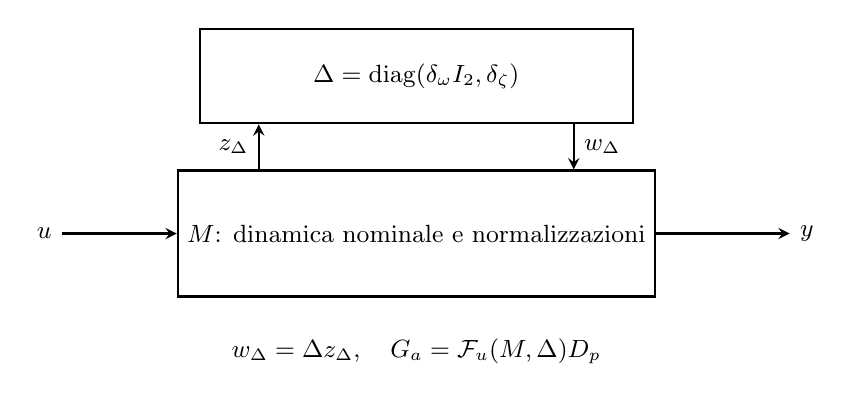
\begin{tikzpicture}[>=stealth,thick,every node/.style={font=\small}]
\node[draw,minimum width=55mm,minimum height=12mm] (d) at (0,2) {$\Delta=\mathrm{diag}(\delta_\omega I_2,\delta_\zeta)$};
\node[draw,minimum width=55mm,minimum height=16mm] (m) at (0,0) {$M$: dinamica nominale e normalizzazioni};
\path (m.north) ++(-2,0) coordinate (mz);
\path (d.south) ++(-2,0) coordinate (dz);
\path (m.north) ++(2,0) coordinate (mw);
\path (d.south) ++(2,0) coordinate (dw);
\draw[->](mz)--(dz) node[midway,left] {$z_\Delta$};
\draw[->](dw)--(mw) node[midway,right] {$w_\Delta$};
\draw[->](-4.5,0)node[left] {$u$}--(m.west);
\draw[->](m.east)--++(1.7,0)node[right] {$y$};
\node at (0,-1.5) {$w_\Delta=\Delta z_\Delta,\quad G_a=\mathcal F_u(M,\Delta)D_p$};
\end{tikzpicture}
